\documentclass[14pt, a4paper]{extarticle}

\usepackage{my_GOST}
\usepackage{hyperref}
\usepackage{listings}
\usepackage{array}
\usepackage{caption}
\hypersetup{
	pdftex,
	colorlinks = true,
	linkcolor = black,
	filecolor = magenta,
	citecolor = green,      
	urlcolor = cyan,
}

% к таблице и листингу подпись сверху, перед каждым иллюстративным материалом анонсировать
% написатьт в квадратных скобках к рекурсии комментарием что это метод и понятно почему вызываем его снова
\definecolor{mylightgray}{RGB}{240,240,240}
\definecolor{mygreen}{rgb}{0,0.6,0}
\definecolor{mygray}{rgb}{0.5,0.5,0.5}
\definecolor{mymauve}{rgb}{0.58,0,0.82}

\lstset{
	backgroundcolor=\color{mylightgray},rulecolor=\color{red},  % choose the background color; you must add \usepackage{color} or \usepackage{xcolor}; should come as last argument
	basicstyle=\footnotesize\ttfamily,        % the size of the fonts that are used for the code
	breakatwhitespace=false,         % sets if automatic breaks should only happen at whitespace
	breaklines=true,                 % sets automatic line breaking
	captionpos=t,                    % sets the caption-position to bottom
	commentstyle=\color{mygreen},    % comment style
	extendedchars=false,              % lets you use non-ASCII characters; for 8-bits encodings only, does not work with UTF-8
	firstnumber=0,                % start line enumeration with line 1000
	frame=shadowbox,
	%rulesepcolor=\color{green},	                   % adds a frame around the code
	keepspaces=true,                 % keeps spaces in text, useful for keeping indentation of code (possibly needs columns=flexible)
	keywordstyle=\color{blue}\textbf,       % keyword style
	language=C++,                 % the language of the code
	morekeywords={*,...},            % if you want to add more keywords to the set
	numbers=left,                    % where to put the line-numbers; possible values are (none, left, right)
	numbersep=5pt,                   % how far the line-numbers are from the code
	numberstyle=\scriptsize\color{mygray}, % the style that is used for the line-numbers
	rulecolor=\color{black},         % if not set, the frame-color may be changed on line-breaks within not-black text (e.g. comments (green here))
	showspaces=false,                % show spaces everywhere adding particular underscores; it overrides 'showstringspaces'
	showstringspaces=false,          % underline spaces within strings only
	showtabs=false,                  % show tabs within strings adding particular underscores
	stepnumber=1,                    % the step between two line-numbers. If it's 1, each line will be numbered
	stringstyle=\color{mymauve},     % string literal style
	tabsize=4,	                   % sets default tabsize to 2 spaces
	title=\lstname                   % show the filename of files included with \lstinputlisting; also try caption instead of title
}
\usepackage{YATPR}

\usepackage[utf8]{inputenc}
\usepackage{amsmath}
\usepackage{float}

\begin{document}
\begin{titlepage}
	\newgeometry{pdftex, left=2cm, right=2cm, top=2.5cm, bottom=2.5cm}
	\fontsize{12pt}{12pt}\selectfont
	\noindent \begin{minipage}{0.15\textwidth}
		
\includegraphics[width=\linewidth]{pictures/b_logo.jpg}
	\end{minipage}
	\noindent\begin{minipage}{0.9\textwidth}\centering
		\textbf{Министерство науки и высшего образования Российской Федерации}\\
		\textbf{Федеральное государственное бюджетное образовательное учреждение высшего образования}\\
		\textbf{«Московский государственный технический университет имени Н.Э.~Баумана}\\
		\textbf{(национальный исследовательский университет)»}\\
		\textbf{(МГТУ им. Н.Э.~Баумана)}
	\end{minipage}
	
	\noindent\rule{18cm}{3pt}
	\newline\newline
	\noindent ФАКУЛЬТЕТ $\underline{\text{«Информатика и системы управления»}}$ \newline\newline
	\noindent КАФЕДРА $\underline{\text{«Программное обеспечение ЭВМ и информационные технологии»}}$\newline\newline\newline\newline\newline\newline\newline
	
	
	\begin{center}
		\Large\textbf{Отчет по лабораторной работе №5}\newline
	\end{center}
	
	\noindent\textbf{Название} $\underline{\text{~Моделирование работы информационного центра~~~~~~~~~}}$\newline\newline\newline
	\noindent\textbf{Дисциплина} $\underline{\text{~Моделирование~~~~~~~~}}$\newline\newline
	\noindent\textbf{Студент} $\underline{\text{Зайцева А. А.~~~~~~~~~~~~~~~~~~~~~~~~~~~~~~~~~~~~~~~~~}}$\newline\newline
	\noindent\textbf{Группа} $\underline{\text{ИУ7-72Б~~~~~~~~~~~~~~~~~~~~~~~~~~~~~~~~~~~~~~~~~~~~}}$\newline\newline
	\noindent\textbf{Оценка (баллы)} $\underline{\text{~~~~~~~~~~~~~~~~~~~~~~~~~~~~~~~~~~~~~~~~~~~~~~~~~}}$\newline\newline
	\noindent\textbf{Преподаватель}$\underline{\text{~Рудаков И. В.~~~~~~~~~~}}$\newline
	
	\begin{center}
		\vfill
		Москва~---~\the\year
		~г.
	\end{center}
 \restoregeometry
\end{titlepage}


\setcounter{page}{2}

\section{Задание}

Промоделировать работу системы массового обслуживания, определить минимальный размер буфера памяти, при котором не будет потерянных заявок. 

Управляющую программу реализовать по двум принципам: $\Delta t$ и событийному. Время появления заявок распределено по равномерному закону, время обработки заявки обслуживающим аппаратом -- по закону Пуассона (вариант из лабораторной работы №1). С заданной вероятностью обработанная заявка возвращается обратно в очередь на обслуживание.



\section{Теоретические сведения}

\subsection{Распределения}

\textbf{Равномерное распределение}

Функция плотности распределения $f(x)$ случайной величины $X$, имеющей равномерное распределение на отрезке $[a, b]$ ($X \sim R(a, b)$), где $a, b \in R$, имеет следующий вид:
\begin{equation}
	f(x)=\begin{cases}
		\frac{1}{b - a}, & x \in [a, b] \\
		0, & \text{иначе}.
	\end{cases}
\end{equation}

Соответствующая функция распределения $F(x) = \int_{-\infty}^{x}f(t)dt$ принимает вид: 
\begin{equation}
	F(x)=\begin{cases}
		0, & x < a \\
		\frac{x - a}{b - a}, & x \in [a, b] \\
		1, & x > b.
	\end{cases}
\end{equation}


\subsection{Распределение Пуассона}

Дискретная случайная величина $X$ имеет закон распределения Пуассона с параметром $\lambda$ ($X \sim \Pi(\lambda)$), где $\lambda > 0$, если она принимает значения $0, 1, 2,...$ с вероятностями:

\begin{equation}
	P(X = k)= e^{-\lambda}\frac{\lambda^{k}}{k!}, \quad k \in \{0, 1, 2, ...\}
\end{equation}

Соответствующая функция распределения принимает вид:

\begin{equation}
	F(x) = P(X < x) = \sum_{k=0}^{x-1}P(X = k) = e^{-\lambda}\sum_{k=0}^{x-1}\frac{\lambda^{k}}{k!} 
\end{equation}

\subsection{Принципы реализации управляющей программы}

Управляющая программа реализуется по следующим стандартным принципам.

\begin{enumerate}
	\item Принцип $\Delta t$. Данный принцип заключается в последовательном анализе состояний всех блоков системы в момент $t + \Delta t$ по заданному состоянию блоков в момент времени $t$. При этом новое состояние блоков определяется в соответствии с их алгоритмическим описанием с учетом действия случайных факторов. В результате анализа принимается решение о том, какие общесистемные события  должны имитироваться на данный момент времени. Основные недостатки: значительные затраты вычислительных ресурсов при малых $\Delta t$ и вероятность пропуска отдельных событий при слишком больших
$\Delta t$, что исключает возможность получения правильных результатов моделирования.
	\item Событийный принцип. При использовании данного принципа состояния всех блоков имитационной модели анализируются лишь в момент появления какого либо события. Момент поступления следующего события определяется минимальным значением из списка будущих событий, представляющего собой совокупность моментов ближайшего изменения состояния каждого из блоков системы
\end{enumerate}

Помимо описанных стандартных принципов также существует комбинированный подход.


\section{Результаты работы программы}

В программе реализованы программные имитаторы источника информации (заявок) и обслуживающего аппарата, а также две управляющие программы, основанные на принципах $\Delta t$ и событийном, соответственно. При заданных параметрах источника информации (параметры $a$ и $b$ равномерного распределения), параметрах обслуживающего аппарата (параметр $lambda\_value$ распределения Пуассона и вероятность повторного попадания в очередь после обработки $p\_reenter$), числе заявок $request\_count$ и шаге $delta\_t$ (для управляющей программы, основанной на принципе $\Delta t$), каждая из управляющих программ моделирует действие системы и выводит максимальную длину очереди за весь период моделирования, чтобы определить минимальный размер буфера памяти, необходимый для того, чтобы не было потерянных заявок.

Для исследования разработанная программа была выполнена при фиксированных параметрах $a=0$, $b=10$, $n\_tasks=1000$, $delta\_t=0.01$ и параметрах $lambda\_value$ и $p\_reenter$, принимающих значения из множеств $\{1, 4, 10\}$ и  $\{0.1, 0.5, 0.9\}$, соотвественно. На рисунке \ref{pic:1} приведена таблица результатов, полученных при описанном исследовании.


\newpage
\begin{figure}[h]
	\begin{center}
		{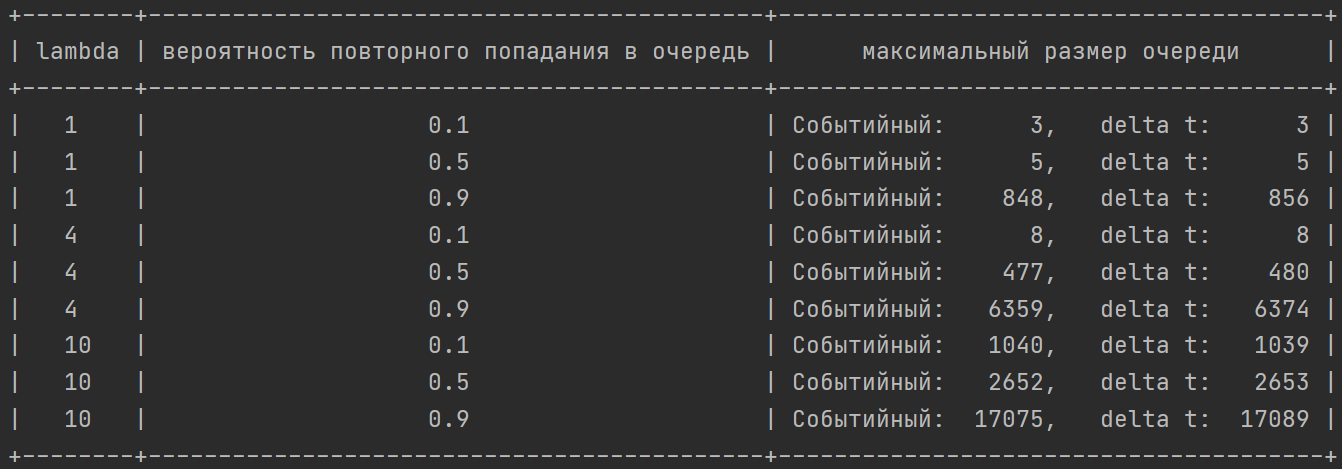
\includegraphics[scale=0.85]{pictures/1.png}
			\caption{Таблица с результатами исследования программы}
			\label{pic:1}}
	\end{center}
\end{figure}

Максимальная длина очереди, полученная различными управляющими программами при одинаковых параметрах различается, так как времена генерации и обработки заявок хоть и распределены по одинаковому закону, но все еще являются случайными величинами.

Максимальная длина очереди растет по мере роста $lambda\_value$ (так как время обработки заявки растет) и $p\_reenter$ (так как все больше заявок попадают в очередь на обслуживание повторно).

\section{Код программы}

В листинге \ref{lst:list1} (используемый язык -- Python) приведен код программных имитаторов источника информации и обслуживающего аппарата. 

\begin{lstlisting}[caption = {Код программных имитаторов источника информации и обслуживающего аппарата}, label=lst:list1]
class RequestsGenerator:
	def __init__(self, a: float, b: float):
		self.a = a
		self.b = b
	
	def get_request_time(self):
		return self.a + (self.b - self.a) * random.random()


class RequestsProcessor:
	def __init__(self, lambda_value, p_reenter: float):
		self.lambda_value = lambda_value
		self.p_reenter = p_reenter
		self.queue_size = 0
		self.max_queue_size = 0
		self.processed_requests = 0
	
	def process_request(self):
		if self.queue_size > 0:
			self.processed_requests += 1
			self.queue_size -= 1
			
			if numpy_random.random_sample() <= self.p_reenter:
				self.add_request_in_queue()
				self.processed_requests -= 1
	
	def get_processing_time(self):
		return poisson.rvs(self.lambda_value, size=1)[0]
	
	def add_request_in_queue(self):
		self.queue_size += 1
		if self.queue_size > self.max_queue_size:
			self.max_queue_size = self.queue_size
	
	def clean_stats(self):
		self.queue_size = 0
		self.max_queue_size = 0
		self.processed_requests = 0
\end{lstlisting}

В листинге \ref{lst:list2} приведен код управляющих программ, основанных на принципах $\Delta t$ и событийном. 

\begin{lstlisting}[caption = {Код управляющих программ, основанных на принципах $\Delta t$ и событийном}, label=lst:list2]
class EventBasedController:
	@staticmethod
	def simulate(generator: RequestsGenerator, processor: RequestsProcessor, request_count):
		gen_next_event_time = generator.get_request_time()
		proc_next_event_time = gen_next_event_time + processor.get_processing_time()
		
		while processor.processed_requests < request_count:
			if gen_next_event_time <= proc_next_event_time:
				processor.add_request_in_queue()
				gen_next_event_time += generator.get_request_time()
			
			else:
				processor.process_request()
				if processor.queue_size > 0:
					proc_next_event_time += processor.get_processing_time()
				else:
					proc_next_event_time = gen_next_event_time + processor.get_processing_time()
		
		return processor.max_queue_size, round(proc_next_event_time)


class DeltaTBasedController:
	@staticmethod
	def simulate(generator: RequestsGenerator, processor: RequestsProcessor, request_count, delta_t):
		gen_next_event_time = generator.get_request_time()
		proc_next_event_time = gen_next_event_time
		current_time = 0
		while processor.processed_requests < request_count:
			if gen_next_event_time <= current_time:
				processor.add_request_in_queue()
				gen_next_event_time += generator.get_request_time()
			
			if current_time >= proc_next_event_time:
				processor.process_request()
				if processor.queue_size > 0:
					proc_next_event_time += processor.get_processing_time()
				else:
					proc_next_event_time = gen_next_event_time + processor.get_processing_time()
			
			current_time += delta_t
		
		return processor.max_queue_size, round(current_time)
\end{lstlisting}

В листинге \ref{lst:list3} приведен код участка программы, с помощью которого проводилось исследование. 

\begin{lstlisting}[caption = {Код участка программы, с помощью которого проводилось исследование}, label=lst:list3]

def simulate_with_params(a, b, lambda_value, reenter_prob, n_tasks, delta_t):
	print()
	print(f'Генератор: R({a}, {b}), ОА: П({lambda_value}), '
	f'вероятность повторного попадания в очередь: {reenter_prob}, число заявок: {n_tasks}, delta t: {delta_t}')
	generator = RequestsGenerator(a, b)
	processor = RequestsProcessor(lambda_value, reenter_prob)
	
	random.seed(0)
	numpy_random.seed(0)
	event_based_result = EventBasedController.simulate(generator, processor, n_tasks)
	
	processor.clean_stats()
	random.seed(0)
	numpy_random.seed(0)
	delta_t_based_result = DeltaTBasedController.simulate(generator, processor, n_tasks, delta_t)
	
	print(f'Событийный принцип:    '
	f'Максимальный размер очереди: {event_based_result[0]}, время окончания моделирования: {event_based_result[1]}')
	print(f'Принцип delta t:       '
	f'Максимальный размер очереди: {delta_t_based_result[0]}, время окончания моделирования: {delta_t_based_result[1]}')
	return event_based_result[0], delta_t_based_result[0]


def main():
	a = 1
	b = 10
	n_tasks = 1000
	delta_t = 0.01
	
	lambda_values = [1, 4, 10]
	reenter_probs = [0.1, 0.5, 0.9]
	
	res_table = PrettyTable(field_names=['lambda', 'вероятность повторного попадания в очередь', 'максимальный размер очереди'])
	for lambda_value in lambda_values:
		for reenter_prob in reenter_probs:
			res_event, res_deltat = simulate_with_params(a, b, lambda_value, reenter_prob, n_tasks, delta_t)
			res_table.add_row([lambda_value, reenter_prob, f'Событийный: {res_event: 6d},   delta t: {res_deltat: 6d}'])
	print()
	print()
	print(res_table)
\end{lstlisting}

\end{document}